\documentclass{article}
\usepackage{graphicx} % Required for inserting images
\usepackage{amsmath}

\title{Assignment 3: Upper and Lower Thresholds of a Hysteresis Comparator}
\author{Moaaz Mostafa Ibrahim \hspace{20pt} 2400862}
\date{}

\begin{document}
\maketitle

We denote the \textit{upper threshold voltage} by $V_h$ and the \textit{lower threshold voltage} by $V_l$. Above $V_h$, the comparator outputs the positive rail voltage $V_s$, and below $V_l$, it outputs the negative rail voltage $-V_s$.\\

\begin{figure}[h]
    \centering
    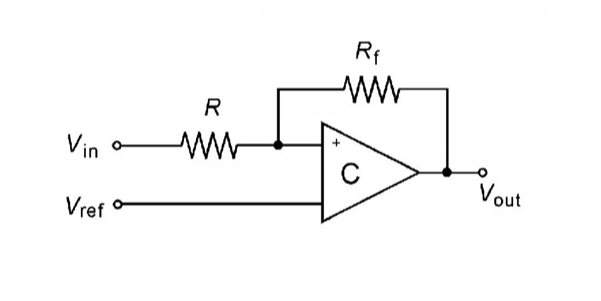
\includegraphics[width=1\linewidth]{Media/Hysteresis.png}
    \caption{Hysteresis Comparator}
    \label{fig:placeholder}
\end{figure}

\section*{Finding $V_h$}
If we assume that $V_{out} = -V_s$, we can obtain the following expression for $V_+$.

\begin{equation*}
    V_+ = V_{in} - \frac{V_{in} - V_{out}}{R_f+R} R = V_{in} - \frac{V_{in} + V_s}{R_f+R} R
\end{equation*}
\noindent
The comparator approaches the positive rail when $V_+ > V_{ref}$, so we substitute $V_+$.

\begin{align*}
    V_{in} - \frac{V_{in} + V_s}{R_f+R} R \ &>\ V_{ref}\\
    \frac{R_f}{R_f+R} V_{in} \ &>\ V_{ref} + \frac{R}{R_f+R} V_s\\
    V_{in} \ &>\ \frac{R_f + R}{R_f} V_{ref} + \frac{R}{R_f} V_s
\end{align*}
\noindent
We have calculated the upper threshold voltage as:
\begin{equation*}
    \boxed{V_h = \frac{R_f + R}{R_f} V_{ref} + \frac{R}{R_f} V_s}
\end{equation*}

\section*{Finding $V_l$}
Now, we assume $V_{out} = V_s$, and again we find an expression for $V_+$.
\begin{equation*}
    V_+ = V_{in} + \frac{V_s - V_{in}}{R_f+R} R
\end{equation*}
\noindent
The comparator approaches the negative rail when $V_+ < V_{ref}$, so we substitute and simplify.
\begin{align*}
    V_{in} + \frac{V_s - V_{in}}{R_f+R} R \ &< \ V_{ref}\\
    \frac{R_f}{R_f+R} V_{in} \ &<\ V_{ref} - \frac{R}{R_f+R} V_s\\
    V_{in} \ &<\ \frac{R_f + R}{R_f} V_{ref} - \frac{R}{R_f} V_s
\end{align*}
\noindent
From that we find the expression for the lower threshold voltage:
\begin{equation*}
    \boxed{V_l = \frac{R_f + R}{R_f} V_{ref} - \frac{R}{R_f} V_s}
\end{equation*}

\end{document}